\documentclass[12pt]{article}
\usepackage{graphicx} % Required for inserting images
\usepackage{amsmath}
\usepackage{url}
\usepackage{amssymb}
\usepackage{fontspec}
\usepackage{cite}
\setmainfont{Times New Roman}
\usepackage[a4paper, margin=2.4cm]{geometry}
\setlength{\parindent}{0pt} % Eliminar sangría
\begin{document}
\begin{center}
\section*{Impulsadores del cambio digital}
HERRERA RODRIGUEZ JONATHAN BENJAMIN
\\SEMINARIO DE TECNOLOGÍAS DE INFORMACIÓN
\\7690-13-1131
\\jbherrerar9@miumg.edu.gt
\end{center}
\section{Resumen}

Todo proceso es un reto y mas cuando se trata de innovar nueva tecnología, la transformación digital es clave no solo para empresas nuevas, sino también para las empresas que no están automatizadas en la tecnología. Las organizaciones deben adoptar tecnologías como la inteligencia artificial, el Internet de las Cosas como IoT y la computación en la nube para competir de manera eficiente y adaptarse a la globalización y las nuevas demandas del mercado. Factores como la preservación del medio ambiente y los cambios en el comportamiento del consumidor también impulsan esta transformación. Las empresas deben adoptar prácticas que reduzcan su huella de carbono y atender al nuevo perfil de clientes, utilizando tecnologías como Big Data y CRM. Además, la transformación digital es clave en sectores como la minería, donde la automatización y tecnologías avanzadas como 5G aumentan la productividad y seguridad. Cloud Computing y las redes de Banda Ancha permiten a cualquier empresa, sin importar su tamaño, acceder a soluciones tecnológicas de vanguardia, fomentando la competitividad global. La transformación digital no implica cambiar el núcleo del negocio, sino mejorar la eficiencia operativa, la atención al cliente y la competitividad mediante la tecnología.

\section{Palabras Clave}
Globalización, Tecnologías emergentes, Big Data, Inteligencia artificial, Minería.

\section{Desarrollo del Tema}

\subsection*{Impulsadores del cambio digital}
Cuando hablamos de transformación digital, seguramente nos viene a la mente los nuevos modelos de negocio, empresas innovadoras, startups, los negocios de entrega a domicilio, nuevos sistemas de pagos, hospedaje, venta y arrendamiento de autos y un gran etcétera. ¿Quiere esto decir que la transformación digital es exclusiva de los nuevos negocios? La respuesta es un rotundo no. La transformación digital por supuesto que debe ser analizada e implementada dentro de los negocios “tradicionales” sin importar su tamaño, ya sea para adecuar sus ofertas y formas de atención al cliente, para competir de manera más ágil con los nuevos competidores, para operar de manera más eficiente, y para mejorar la seguridad y bienestar de sus colaboradores.
El mundo de los negocios se está tornando cada vez más competitivo y está siendo afectado por la tecnología que está habilitando a un sinnúmero de nuevas empresas, pero existen otras fuerzas que igualmente están afectando el mundo de los negocios:
\begin{itemize}
    \item La globalización -que lleva varios años entre nosotros- abre puertas para participar y competir en otras geografías, pero trae consigo a competidores adicionales a nuestros mercados tradicionales. Para aumentar la competitividad no es suficiente con digitar algunas tareas dentro de las empresas, es necesario adecuar procesos operativos mediante el uso de herramientas digitales para ser más ágiles y eficientes, por ejemplo, tecnologías como Blockchain que permitan integrarse a cadenas globales de suministro.
    \item La preocupación por la preservación del medio ambiente también está generando que las empresas estén buscando formas de operar con menor impacto al medio ambiente (disminución de huella de carbono) por mutuo propio o bien por necesidad ante nuevos requerimientos de sus clientes. Si bien este es un reto mayúsculo a nivel global, cada empresa debe hacer su contribución, de lo cual resultarán beneficios directos también para cada una. La reducción de huella de carbono se puede atacar por dos vías directas, reduciendo el consumo de energía (eléctrica) y/o mediante el uso de energías renovables (fotovoltaica, PV), en ambos casos la incorporación de tecnología digital es de gran ayuda para mejorar los procesos de transformación en el manejo, uso y administración de la energía, que es factible gracias a la digitalización de los procesos.
    \item Los cambios en el comportamiento de la sociedad y el uso extensivo de medios electrónicos principalmente en los jóvenes, provocan también cambios para atender al nuevo perfil de cliente. Pareciera que este es uno de los cambios más visibles para todos, aún para aquellos ajenos a la tecnología, pero más allá de su visibilidad es un profundo cambio en la forma de operar para muchas empresas, no es suficiente tener presencia en internet o tener un marketplace. La atención del nuevo perfil de clientes demanda nuevos procesos de atención basados en profundo conocimiento del cliente, agilidad en procesos de manufactura y logística, multicanalidad y en muchos casos omnicanalidad en la atención. Estos cambios requieren de la incorporación nuevas tecnologías como Big Data, Inteligencia Artificial, CRM, entre otras, así como la adecuación de los procesos operativos de cada empresa.
    \item La necesidad y preocupación global por el bienestar de los empleados, sobre todo en entornos de alto peligro (minas, plataformas en alta mar, etc.). Seguramente la mayoría de las personas que estén leyendo este artículo se encuentran en entornos urbanos llevando a cabo trabajos de baja peligrosidad, pero a la fecha siguen existiendo, y son necesarios, trabajos de alto riesgo tales como la minería, por mencionar uno. Entornos como esos tradicionalmente se han llevado a cabo sin el empleo de TIC´s por su lejanía de las redes de comunicaciones tradicionales, sin embargo, las capacidades que brindan las nuevas tecnologías como 5G, permiten llevar conectividad a esos lugares e incorporar soluciones que no solo contribuyen a disminuir el riesgo de los trabajadores, sino aumentan la productividad en ellas. Al hablar de autos autónomos o de conducción remota, lo imaginamos normalmente con ambientes urbanos existiendo diversas iniciativas en diferentes partes del mundo para su desarrollo, pero esos esquemas ya empiezan a ser realidad en la minería, se tienen ejemplos en algunos países (China, Rusia) donde se ha incorporado tecnología de Realidad Aumentada (AR) y robótica mediante redes 5G a los equipos de transporte y excavación dentro de las minas tanto a cielo abierto como subterráneas, disminuyendo significativamente los riesgos de salud para los trabajadores, pero también aumentando la productividad. Por ejemplo, los grandes camiones dentro de las minas aumentaron en 17\% su velocidad promedio, a la vez de bajar el índice de incidentes de manera significativa. De esta forma, las operaciones de extracción aumentan la productividad al requerir menos personal en el sitio disminuyendo los tiempos muertos propios de operación manual (transporte, descansos, etc.).
\end{itemize}

Sin duda la transformación digital es una poderosa herramienta para lidiar con todos los escenarios planteados anteriores, no es algo inherente a nuevas empresas únicamente. Todas las empresas, sin importar su giro o tamaño, tienen procesos operativos, de transformación, de atención a clientes y logística, que son sujetos de transformarse digitalmente para lograr mayor agilidad, eficiencia operativa y eficiencia en costos. Hago énfasis en el tamaño de las empresas, ya que la transformación digital no solo está al alcance de las grandes empresas, las nuevas tecnologías están al alcance de todo tipo (en cuanto a tamaño) de empresas.

Cloud Computing (servicios de cómputo en la nube) ha hecho realidad que cualquier empresa pueda acceder a tecnología de punta sin hacer grandes inversiones de capital, accediendo no solo a poder de cómputo sino accediendo a entornos tecnológicos completos (PAAS Plataform as a Service) para desarrollar soluciones basadas en Big Data, Inteligencia Artificial, Blockchain. Por supuesto no debemos olvidar que la tecnología que nos permite conectar esos servicios cloud es la Bandas Ancha, hoy en día con servicios FTTx y mBB. Sumando estás dos tecnologías (cloud y Banda Ancha) con las ideas y procesos de negocio viables basados en TIC´s, cualquier empresa puede competir de tu a tu con empresas de todo el mundo y acelerar su crecimiento.

Todas las empresas deben plantearse la transformación digital, lo que no significa necesariamente cambiar de fondo su objetivo de negocio, implica mejorar sus procesos operativos dentro de su negocio para mejorar su competitividad y atención a sus clientes, haciendo uso de tecnologías digitales.
\cite{UNAMRevista}, \cite{AmericaEconomia}
\begin{figure}[h]
    \centering
    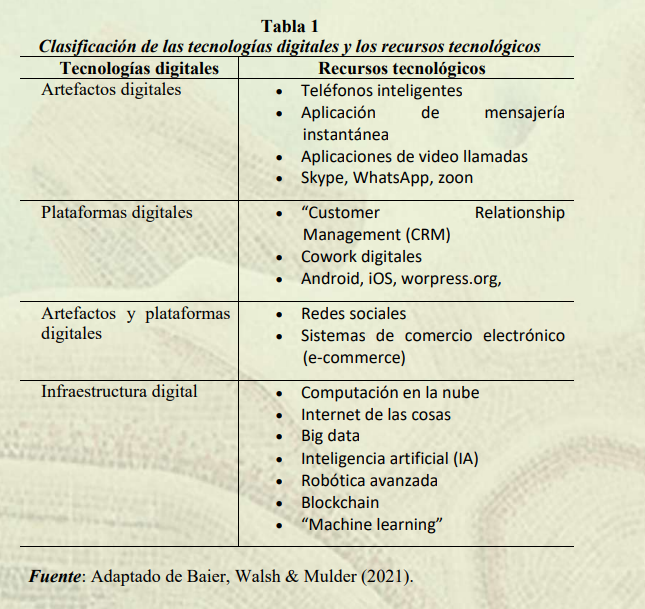
\includegraphics[width=1\textwidth]{Figura1.png}
    \caption{Clasificacion de las tecnologias digitales y los recursos tecnológicos}
    \label{fig:imagen1}
\end{figure}

\begin{figure}[h]
    \centering
    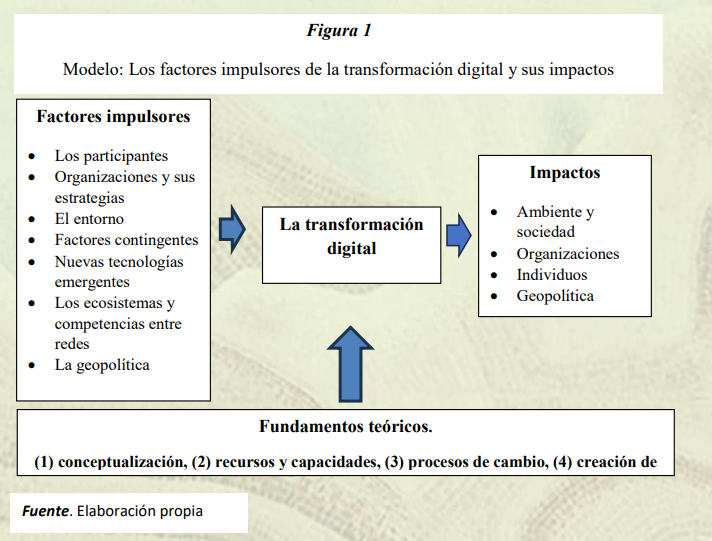
\includegraphics[width=1\textwidth]{Figura2.png}
    \caption{Transformación Digital}
    \label{fig:imagen2}
\end{figure}

Los impulsadores del cambio digital son factores y tendencias que fomentan la adopción y evolución de tecnologías digitales en organizaciones y sociedades. Aquí te presento algunos de los principales:
\begin{enumerate} 
\item Innovación Tecnológica: La rápida evolución de tecnologías como la inteligencia artificial, el Internet de las Cosas (IoT), la computación en la nube, y el análisis de datos impulsa la transformación digital al ofrecer nuevas herramientas y capacidades.
\item Demanda de Mejora de la Experiencia del Cliente: Las expectativas crecientes de los clientes para experiencias más rápidas, personalizadas y convenientes obligan a las empresas a adoptar tecnologías digitales para satisfacer esas demandas.
\item Competencia en el Mercado: La necesidad de mantenerse competitivo en un mercado cada vez más digitalizado impulsa a las organizaciones a adoptar nuevas tecnologías para mejorar su eficiencia, reducir costos y ofrecer mejores productos o servicios.
\item Automatización de Procesos: La capacidad de automatizar tareas repetitivas y procesos empresariales mediante tecnologías digitales permite a las organizaciones mejorar la eficiencia operativa y reducir errores humanos.
\item Acceso a Datos y Análisis Avanzado: La disponibilidad de grandes volúmenes de datos y herramientas de análisis avanzado permite a las empresas tomar decisiones basadas en datos más precisos y relevantes.
\item Cambio en el Modelo de Trabajo: La creciente tendencia hacia el trabajo remoto y flexible ha acelerado la necesidad de soluciones digitales que faciliten la colaboración y la comunicación en entornos distribuidos.
\item Regulaciones y Políticas: Las normativas y políticas gubernamentales relacionadas con la protección de datos, ciberseguridad y digitalización también pueden actuar como impulsores del cambio digital.
\item Globalización: La interconexión global facilita la transferencia de conocimientos y tecnologías, impulsando la adopción digital en diversas regiones y sectores.
\item Inversión y Financiación: La disponibilidad de capital para inversiones en tecnología y la financiación de iniciativas digitales puede acelerar la adopción de nuevas tecnologías en las empresas.
\item Cambio Cultural: La evolución de la mentalidad organizacional hacia la adopción de la tecnología y la cultura digital también juega un papel crucial en la transformación digital.
\end{enumerate}
Estos factores suelen actuar en conjunto, creando un entorno propicio para la transformación digital y la adopción de nuevas tecnologías.
\cite{mckinsey2020}

\subsection*{Observación}
\begin{enumerate}
    \item El impacto ambiental es un impulsor clave de la transformación digital. 
    \item El uso de tecnologías emergentes permite una operación más ágil y segura en entornos peligrosos.
    \item La digitalización es clave para reducir la huella de carbono y mejorar la sostenibilidad empresarial.
\end{enumerate}

\subsection*{Comentario}
\begin{enumerate}
    \item Hoy en día es muy importante que las empresas tradicionales aprovechen la transformación digital para mantenerse competitivas en el mercado actual, se ve que innovan en hacer promociones en redes sociales pero aun esas tecnologías le pueden sacar aun mas provecho para impulsar negocios. 
    \item La adopción de tecnologías como 5G y cloud computing permite aumentar la eficiencia y disminuir riesgos, especialmente en sectores peligrosos.
\end{enumerate}

\section*{Conclusiones}
\begin{enumerate}
    \item Si nos enfocamos en la adaptación digital en las empresas de cualquier capacidad, permitiéndoles mejorar su eficiencia operativa y mantenerse competitivas en un mundo cada vez más globalizado. No solo afecta la operación interna, sino también la forma en que interactúan con sus clientes, mejorando la experiencia del consumidor.
    \item La inteligencia artificial y Big Data, ofrecen herramientas poderosas para optimizar procesos, reducir costos y tomar decisiones basadas en datos precisos. Esto brinda a las empresas la capacidad de adaptarse rápidamente a los cambios del mercado.
    \item Pasarnos al tema de la digitalización podemos decir que también promueve la sostenibilidad al incorporar prácticas que reducen la huella de carbono y el consumo de energía. Las empresas no solo aumentan su eficiencia, sino que también contribuyen a la preservación del medio ambiente, respondiendo a demandas sociales y regulaciones gubernamentales.
\end{enumerate}

\bibliographystyle{plain}
\bibliography{referencias}

\section*{Repositorio Git}
\begin{itemize}
    \item \url{https://github.com/JohnH31/SEMINARIO-DE-TECNOLOG-AS-DE-INFORMACI-N.git}
\end{itemize}

\end{document}
